%\section{Аналіз існуючих моделей і алгоритмів управління логістичними системами. Постановка задачі}
\section{Аналіз предметної області}
\subsection{Розподільча логістична система як об'єкт дослідження}
% https://essuir.sumdu.edu.ua/bitstream/123456789/38038/1/Bilovodska_Kyslyi_Olefirenko_Solyanyk.pdf
Розподільча логістика --- це частина загальної логістичної системи, яка забезпечує найбільш ефективну організацію розподілу продукції, охоплюючи систему товароруху і виконуючи логістичні операції транспортування, складування, упакування та ін.~\cite{Kusluy2010}.

Розподільча логістика спрямована на комплексне планування, управління та фізичне опрацювання потоку готових виробів у супроводі необхідного інформаційного, фінансового та сервісного потоку від моменту здачі-приймання товарів з виробництва до замовника (споживача) з метою оптимізації витратних та часових характеристик зазначеної частини матеріального і нематеріального потоків.
Головна мета розподільчої логістики --- організація розподільчої діяльності відповідно до замовлень клієнтів з мінімальними загальними витратами~\cite{Kusluy2010}.

Принципова відмінність розподільчої логістики від традиційного розуміння збуту полягає насамперед у системному взаємозв'язку процесу розподілу з процесами виробництва і закупівель під час управління матеріальними потоками, а також системному взаємозв'язку всіх функцій всередині самого розподілу.

Матеріальний потік у сфері розподілу має форму готової продукції.
Залежно від суб'єкту економічних відносин, який бере участь у доведенні ресурсів до споживача, потік готової продукції можна подати як товарний потік або як вантажний потік (на транспорті).

Розподільча логістика будується на загальних логістичних принципах~\cite{Anikin1999}:
\begin{itemize}
	\item координація всіх процесів товароруху, починаючи від кінцевих операцій товаровиробника та закінчуючи сервісом споживача;
	\item інтеграція всіх функцій управління процесами розподілу готової продукції та послуг, починаючи від визначення мети та закінчуючи контролем;
	\item адаптація комерційного, канального та фізичного розподілу до постійно змінних вимог ринку та потреб споживача;
	\item координація всіх процесів товароруху, починаючи від кінцевих операцій товаровиробника та закінчуючи сервісом споживача;
	\item системність як управління розподілом в його цілісності та взаємозалежності всіх елементів збутової діяльності;
	\item комплексність, тобто вирішення всієї сукупності проблем, пов’язаних із задоволенням платоспроможного попиту покупців;
	\item оптимальність стосовно як елементів системи, так і режиму її функціонування;
	\item раціональність як в організаційній структурі, так і в організації управління.
\end{itemize}

Склад завдань розподільчої логістики на мікро- та на макрорівні різний~(таблиця~\ref{tab:logistic_functions}).

\begin{table}[H]
	\caption{Завдання розподільчої логістики на мікро- та макрорівнях}
	\label{tab:logistic_functions}
	\begin{tabular}{@{}|p{0.53\linewidth}|p{0.4\linewidth}|@{}}
		\hline
		Мікрорівень & Макрорівень \\ \hline
		\begin{itemize}[leftmargin=*]
			\item оптимізація формування портфеля замовлень;
			\item укладання договорів із замовниками на постачання продукції;
			\item забезпечення ритмічності та дотримання планомірності реалізації продукції;
			\item вивчення і задоволення потреб у логістичному сервісі;
			\item раціоналізація параметрів, структури і просування динамічних матеріальних потоків;
			\item оптимізація параметрів і умов зберігання запасів товарного характеру;
			\item формування і вдосконалення системи інформаційного забезпечення.
		\end{itemize}
		            &
		\begin{itemize}[leftmargin=*]
			\item вибір схеми розподілу матеріального потоку;
			\item визначення оптимальної кількості розподільчих центрів на території, яка обслуговується;
			\item визначення оптимального місця розташування розподільчого центру на території, яка обслуговується, та ін.
		\end{itemize} \\ \hline
	\end{tabular}
\end{table}

\subsection{Проблеми моделювання і управління розподільчими логістичними системами}
Основною проблемою, характерною для об'єкта дослідження, яка породжує безліч інших проблем, є його ієрархічність і розподіленість.
В таких системах процеси розосереджені по окремих підсистемах і знаходяться на різних рівнях ієрархії.
Для таких систем вирішується комплекс взаємопов'язаних задач в режимі багатосторонньої взаємодії між менеджерами-аналітиками, що відповідають за окремі локальні завдання і \acrshort{computer}.
Основними ознаками розподіленості будь-якої логістичної системи можна вважати:
\begin{itemize}
	\item наявність механізму розбиття даної системи на окремі взаємопов'язані підсистеми;
	\item окремі складові системи географічно відокремлені;
	\item відносна автономність окремих підсистем;
	\item спільне завдання всієї системи розглядається у вигляді набору окремих локальних підзадач;
	\item паралельність і асинхронність рішення окремих локальних задач різними виконавцями.
\end{itemize}

Першою проблемою, яку необхідно вирішувати, є розбиття кожної системи на окремі локальні підсистеми.
Можна сказати, що формалізація цих двох завдань здійснюється на основі декомпозиції і агрегування.
Декомпозиція полягає в розчленуванні вихідної задачі на ряд відносно незалежних підзадач, а агрегування --- в заміні окремих груп змінних, що характеризують ефективність функціонування системи, змінними-агрегатами.
При цьому висувається вимога повної (достатньої) еквівалентності задач.
Агрегування параметрів і змінних здійснюється в ході руху вгору по ієрархії.
Це пов'язано з великою розмірністю завдання і неможливістю прийняття рішень на основі варіювання всіх параметрів і змінних.
Основні ідеї, які реалізуються при синтезі моделі на основі декомпозиції і агрегування полягають у наступному:
\begin{itemize}
	\item нехтуючи слабкими зв'язками між окремими підсистемами, зробити декомпозицію;
	\item використовуючи трохи відмінності між ними, зробити агрегування;
	\item використовуючи сильні відмінності, виділити <<вузькі місця>>, відкинувши на основі апріорних оцінок несуттєві обмеження.
\end{itemize}

\subsection{Моделі логістичних систем}
Моделювання в загальному вигляді являє собою один з основних методів пізнання, є формою відображення дійсності і полягає у з'ясуванні або відтворенні тих чи інших властивостей реальних об'єктів, процесів, явищ за допомогою абстрактного опису у вигляді зображення, плану, карти, сукупності рівнянь, алгоритмі і програм.

Одним з найбільш ефективних методів дослідження складних систем розподільчої логістики є імітаційне моделювання~\cite{Kobelev2003}.

Імітаційне моделювання --- експериментальний метод дослідження реальної системи за її імітаційною моделлю, який поєднує особливості експериментального підходу і специфічні умови використання обчислювальної техніки~\cite{Emelyanov2002}.

Серед переваг імітаційного моделювання відзначають~\cite{Emelyanov2002}:
\begin{enumerate}
	\item Відображення динамічних процесів і поведінкових аспектів зовнішнього середовища.
	\item Можливість виявлення закономірностей, динамічних тенденцій розвитку і функціонування складної системи в умовах неповної та неточної інформації.
	\item Опис взаємодії та поведінки безлічі активних агентів в соціальних системах.
	\item Реалізацію принципів об'єктно-орієнтованого проектування і застосування високотехнологічних рішень при побудові комп'ютерних моделей та ін.
\end{enumerate}

Головною проблемою при побудові будь імітаційної моделі є необхідність побудови комплексних математичних моделей і розробки програмного коду імітаційної моделі.

У імітаційному моделюванні виділяють такі основні підходи:
\begin{itemize}
	\item системна динаміка;
	\item дискретне моделювання;
	\item агентне моделювання.
\end{itemize}

\subsubsection{Системна динаміка}
Як методологія системна динаміка була запропонована в 1961 році Дж. Форрестером в якості інструменту дослідження інформаційних зворотних зв'язків у виробничо-господарської діяльності.
Процеси, що відбуваються в реальному світі, в системній динаміці представляються в термінах накопичувачів і потоків між ними.
Системнодинамічна модель описує поведінку системи та її структуру як безліч взаємодіючих зворотних зв'язків і затримок.
Математично така модель виглядає як система диференціальних рівнянь.
Результатом моделювання в системній динаміці є виявлення глобальних залежностей і причинно-наслідкових зв'язків у досліджуваній системі~\cite{Shamrin2016}.

\subsubsection{Дискретне моделювання}
Основний об'єкт в системі дискретного моделювання --- пасивний транзакт, який може певним чином представляти собою працівників, деталі, сировину, документи, сигнали і т. п.
Переміщаючись по моделі, транзакти стають в черги до одноканальним і багатоканальним пристроям, захоплюють і звільняють їх, розщеплюються, знищуються і т. д.
Відмінною особливістю даного підходу є час просування по моделі: або від події до події, або через дискретні проміжки часу.
Дискретне моделювання застосовується, якщо можливо припустити, що змінні в системі змінюються миттєво в певні проміжки часу.
Даний підхід імітаційного моделювання є одним з найпоширеніших і застосовується для дослідження соціально-економічних, технічних, логістичних та інших процесів.
На основі дискретного підходу реалізовано найбільше
число систем імітаційного моделювання~\cite{Shamrin2016}.

\subsubsection{Агентне моделювання}
Агентське моделювання з'явилося в 90-х роках і використовується для дослідження децентралізованих систем, динаміка функціонування яких визначається не глобальними правилами і законами (як в інших парадигмах моделювання), а коли ці глобальні правила і закони є результатом індивідуальної активності членів групи.

Агентно-орієнтована система може складатися з одного агента (наприклад, програмний секретар~\cite{Maes1995}), проте весь потенціал розкривається з використанням мультиагентної системи~\cite{Waters1989}.
Під агентом розуміється система, яка має такі властивості~\cite{Jennings1998,Wooldridge1995}:
\begin{enumerate}[label={\arabic*)}]
	\item автономність: агенти мають внутрішній стан (який недоступний іншим агентам) та приймають рішення на основі своїх даних, без прямого втручання людини;
	\item реактивність: агенти розміщуються в навколишньому середовищі (яке може бути фізичним світом, множиною інших агентів, інтернетом і т.д.), здатні спостерігати і своєчасно реагувати на зміни;
	\item проактивність: агенти не тільки реагують на зміни в зовнішньому середовищі, вони здатні виявляти ініціативу для досягнення своєї мети;
	\item соціальність: агенти взаємодіють з іншими агентами (і, можливо, людиною) через спеціальний інтерфейс для досягнення їх цілей.
\end{enumerate}

Мета агентських моделей --- отримати уявлення про ці глобальні правила, загальну поведінку системи, виходячи з припущень про індивідуальну, приватну поведінку її окремих активних об'єктів і взаємодію цих об'єктів в системі.
У разі моделювання логістичних систем, що містять великі кількості активних об'єктів (людей, машин, підприємств чи навіть проектів, активів, товарів і т. п.), які об'єднує наявність елементів індивідуальної поведінки, агентське моделювання є підходом більш універсальним і потужним, оскільки дозволяє врахувати будь-які складні структури та їх поведінку~\cite{Shamrin2016}.

\subsection{Визначення та типи агентів в агентному моделюванні}
Не існує чіткого визначення того, що таке агент. Література пропонує різноманітні визначення, від простих до довгих і вимогливих.
Замість перерахування та розробки різних визначень тут даються два визначення агента [1] та [2], оскільки вони здаються досить загальними, широко прийнятими різними дослідницькими спільнотами та найбільш близькими до агентного моделювання. У [1] агент визначається наступним чином:
<<Агент - це все, що сприймає своє середовище за допомогою датчиків і діє на це середовище через ефектори>>.

Згідно з цим визначенням агентом є будь-яка сутність (фізична чи віртуальна), яка сприймає своє оточення та взаємодіє з ним.
Фізична сутність, яка може розглядатися як агент, - це, у випадку енергосистеми, просте захисне реле або будь-який контролер, який безпосередньо керує певним компонентом енергосистеми або частиною системи.

Віртуальна сутність, яку можна розглядати як агент, - це програмне забезпечення, яке отримує вхідні дані з навколишнього середовища і обчислює результати, які ініціюють дію над ним.

Часто агент - це комбінація фізичної (архітектури обчислень) та віртуальної (частина програмного забезпечення, що працює на обчислювальній архітектурі).
Більш широке зазначеного вище визначення агента, дане в [2],
<<Автономні агенти - це обчислювальні системи, які знаходяться у якомусь складному динамічному середовищі, відчувають і діють самостійно в цьому середовищі і тим самим реалізують набір цілей або завдань, для яких вони розроблені>>

Основною відмінністю цього визначення щодо першого є слова: обчислювальний, самостійність та цілі. Обчислювальні агенти, які нас цікавлять в інженерії програмного забезпечення, відрізняються від біологічних агентів (людей, тварин, бактерій), хоча з першого визначення це розрізнення не очевидно. Автономія (самостійність) означає, що обчислювальні агенти діють без прямого втручання деяких інших суб'єктів і мають певний контроль за своїми діями. Призначення цілі агенту означає, що діяти на навколишнє середовище слід з метою досягнення певної визначеної мети і що агенти виявляють певну раціональну поведінку в навколишньому середовищі. Поведінка тут означає дію, яка виконується після отримання сенсорних входів (або будь-якої послідовності сенсорних входів) [1].
Загальна структура агента проілюстрована на рисунку~\ref{fig:agent_general}.

\begin{figure}[H]
	\centering
	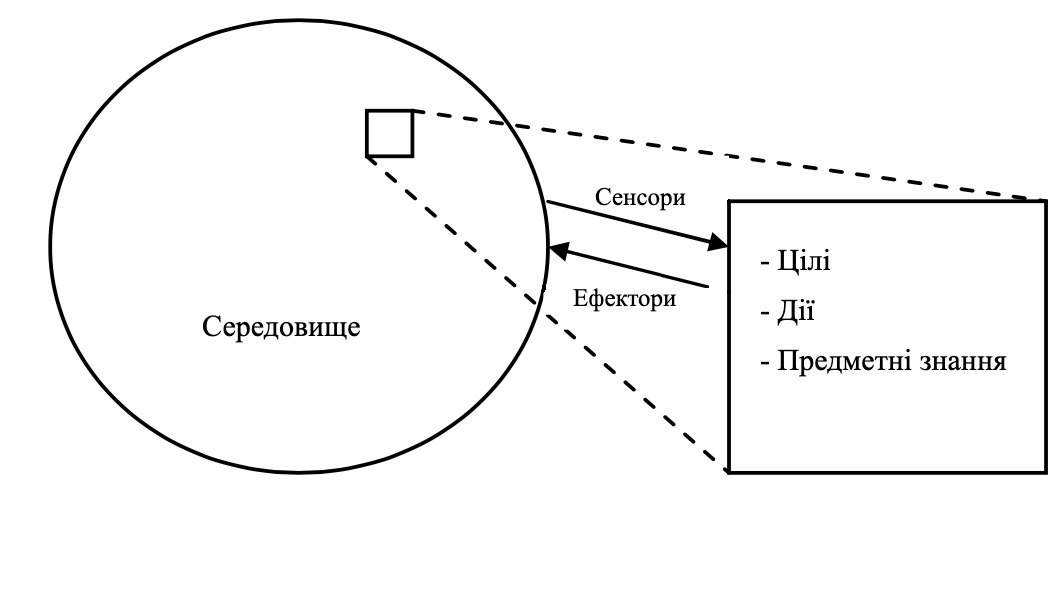
\includegraphics[width=0.8\textwidth]{agent_general}
	\caption{Загальна структура агента}
	\label{fig:agent_general}
\end{figure}

На додаток до сенсорних входів, дій та цілей агент може включати доменні знання (знання про певне середовище або проблему, яку потрібно вирішити). Ці знання можуть бути алгоритмічними, методами штучного інтелекту (AI), заснованими на правилах, нечіткими, нейронними мережами, машинним навчанням, евристикою тощо. У випадку AI агент часто називають інтелектуальним.

Поняття навколишнього середовища, в якому агент мешкає (знаходиться або розміщений у ньому), включає фізичні системи (як в техніці), операційну систему, Інтернет або, можливо, деякі з цих систем разом.

Якщо агент просто своєчасно реагує на зміни зовнішнього середовища і реактивно перетворює свої чуттєві входи на дії, цей агент відомий як реактивний (іноді його називають рефлекторним агентом). Реактивні агенти зазвичай не підтримують внутрішній стан (простий приклад внутрішнього стану - це збереження набору попередніх сенсорних входів) агента і не прогнозують ефект дії. Бо можна сказати, що якщо агент прогнозує ефект дії, він не є реактивним (мається на увазі, що реактивний агент також може підтримувати свій внутрішній стан).

З іншого боку, якщо агент підтримує внутрішній стан, передбачуючи наслідки своїх дій, або, загалом, включає в себе своєрідне міркування, цей агент поводиться свідомо і називається дорадчим агентом.

На рисунку~\ref{fig:agent_reactive} зображена схема реактивного агента. Деякі з авторів не присвоюють жодних цілей реактивним агентам, але цілі можуть бути втілені в правилах обробки сенсорних входів або правилах дії.
На рисунку~\ref{fig:agent_deliv} зображена схема дорадчого агента.

\begin{figure}[H]
	\centering
	\begin{subfigure}[b]{0.49\textwidth}
		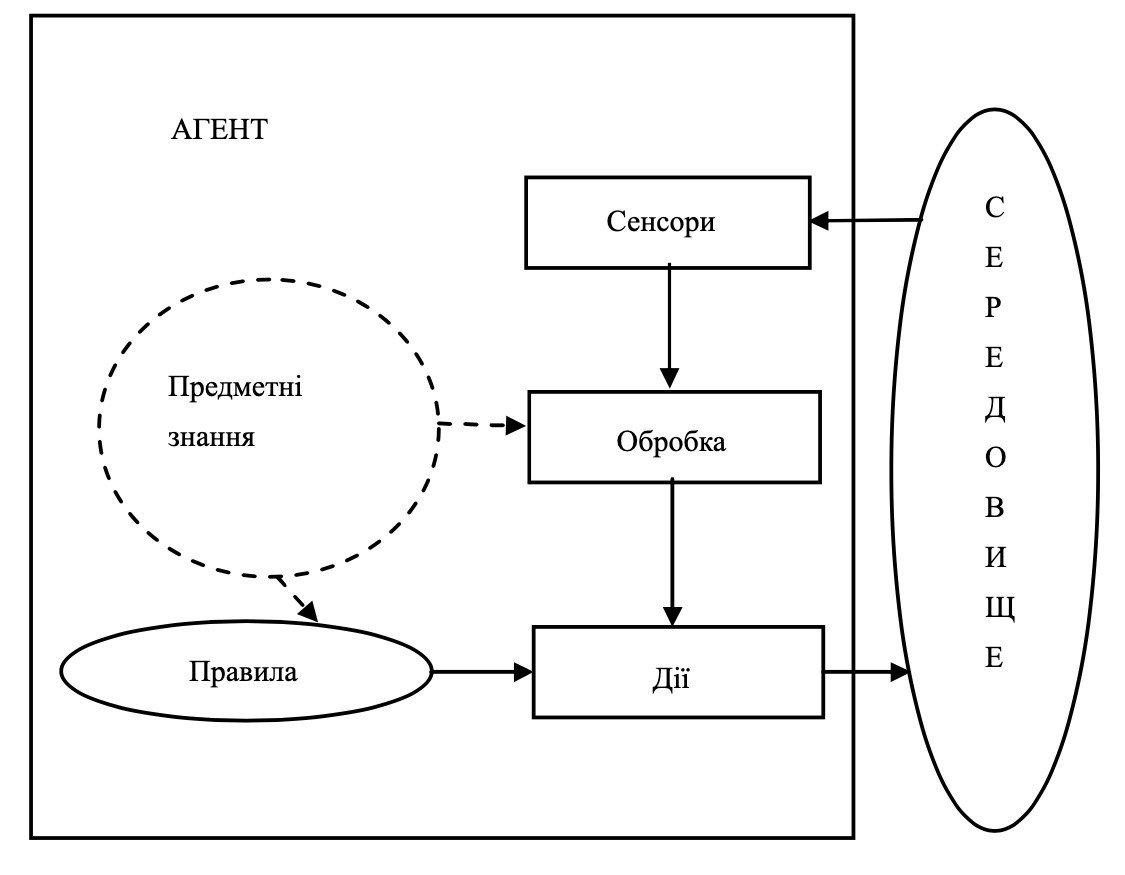
\includegraphics[width=\linewidth]{agent_reactive}
		\caption{Схема реактивного агенту}
		\label{fig:agent_reactive}
	\end{subfigure}
	~
	\begin{subfigure}[b]{0.49\textwidth}
		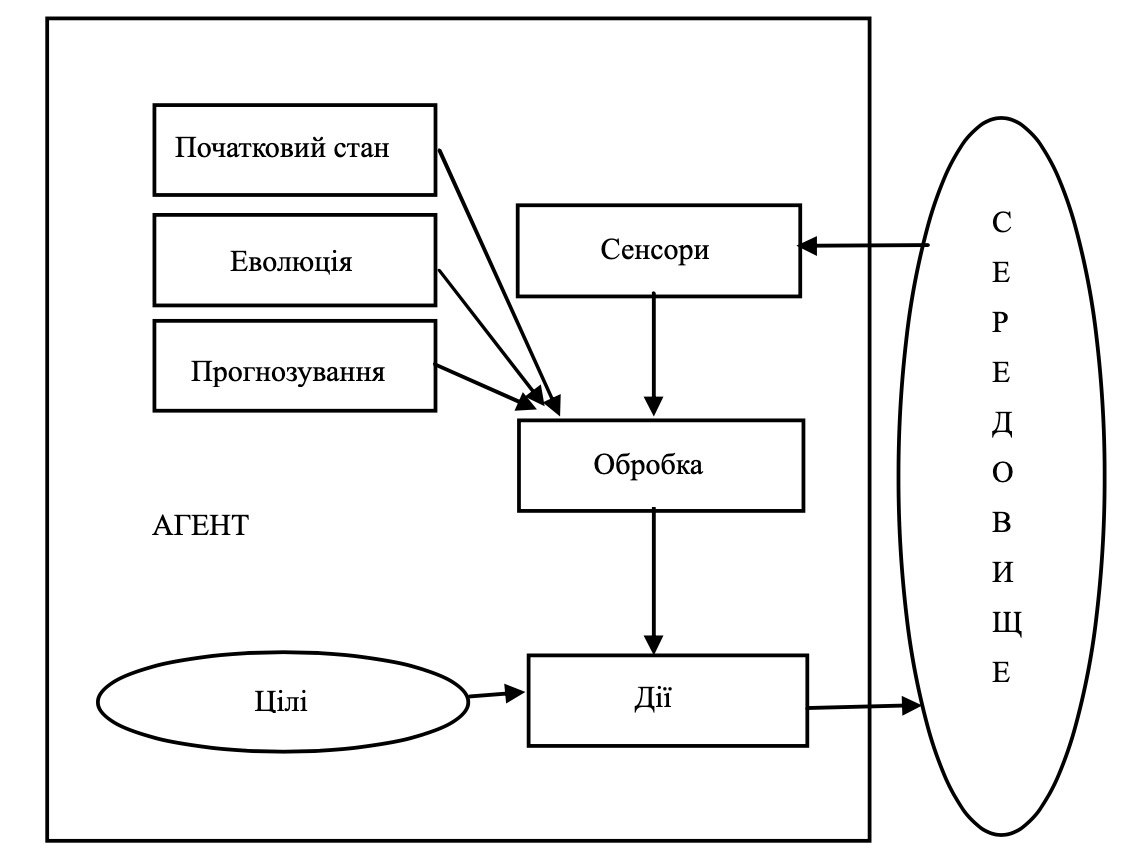
\includegraphics[width=\linewidth]{agent_deliv}
		\caption{Схема дорадчого агенту}
		\label{fig:agent_deliv}
	\end{subfigure}
    \caption{Порівняльна схема агентів}
\end{figure}

Різні визначення агентів передбачають безліч властивостей агента, і агенти зазвичай класифікуються на основі цих властивостей.
У таблиці~\ref{tab:agent_props} перераховано властивості агентів.

{
\tabulinesep=1.2mm
\begin{longtabu} to \textwidth {|X[1,l]|X[3,l]|}
	\caption{Властивості агентів}
	\label{tab:agent_props} \\
	\hline
	Властивість & Значення \\
	\hline
	\endfirsthead
	\caption*{Закінчення таблиці \thetable{}}\\
	\hline
	Властивість & Значення \\
	\hline
	\endhead

	Реактивний & Вчасно реагує на зміни навколишнього середовища \\ \hline
	Автономний & Здійснює контроль за власними діями \\ \hline
	Цілеспрямований & Діє, керуючись певною ціллю, у відповідь на навколишнє середовище \\ \hline
	Тимчасово неперервний & Безперервний процес \\ \hline
	Комунікативний & Спілкується з іншими агентами \\ \hline
	Той, що навчається & Змінює свою поведінку, виходячи з попереднього досвіду \\ \hline
	Мобільний & Здатний транспортувати себе з однієї машини на іншу (це пов'язано переважно з програмними агентами) \\ \hline
	Гнучкий & Діє не за сценарієм \\ \hline
\end{longtabu}
}

\subsection{Мультиагентна система}
Для визначення терміну мультиагентної системи запропоновано різні дефініції,  залежно від наукової дисципліни, з якої вона походить. Єдине та найбільш загальне визначення мультиагентної системи надано нижче.

Мультиагентна система (\acrshort{mas}) - це нещільно поєднана мережа суб'єктів (агентів), що вирішують проблеми, працюють разом, щоб знайти шляхи вирішення проблем, що виходять за межі індивідуальних можливостей або знань кожного суб'єкта (агента)[3].

Той факт, що агенти \acrshort{mas} працюють разом, означає, що має бути визначена співпраця між окремими агентами. Однак концепція співпраці в \acrshort{mas} є в кращому випадку незрозумілою і в гіршому - дуже непослідовною, так що термінологія, можливі класифікації тощо є ще більш проблематичними, ніж у випадку з агентами, що робить будь-яку спробу представити \acrshort{mas} важкою проблемою.
Типологія співпраці з [4] видається найпростішою, і ця типологія використовуються як основа для класифікації \acrshort{mas}. Типологія наведена на рисунку~\ref{fig:mas_topology}.

\begin{figure}[H]
	\centering
	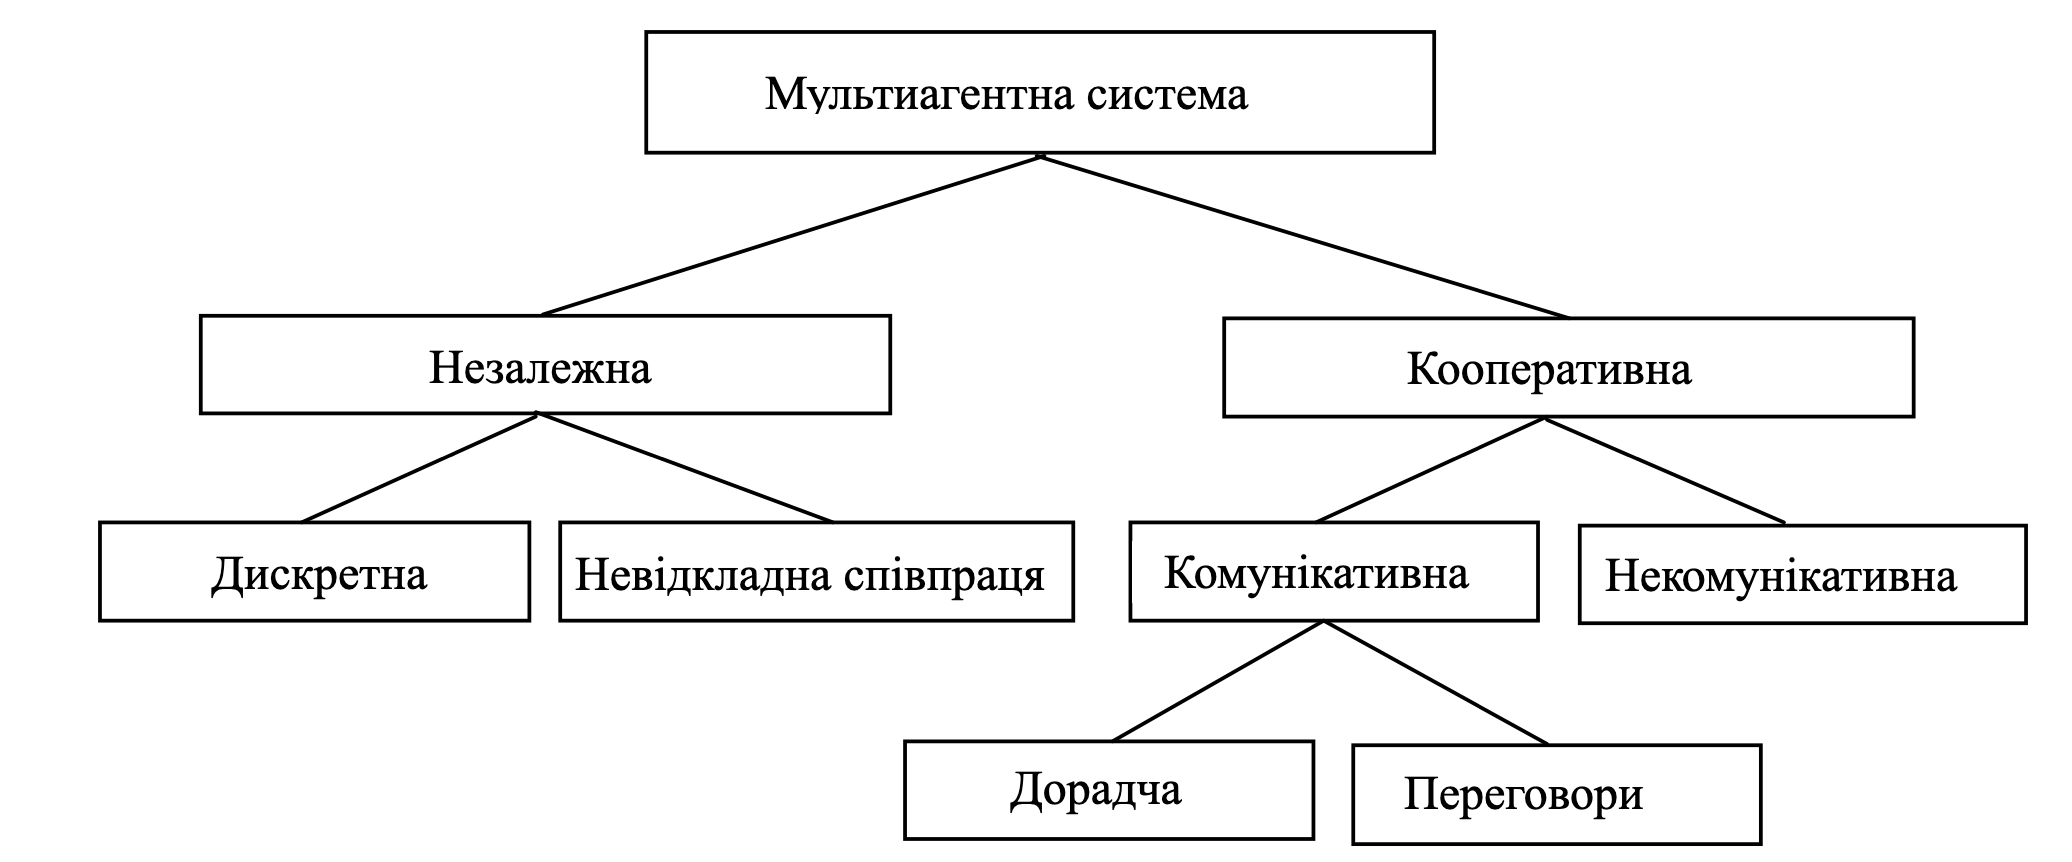
\includegraphics[width=0.8\textwidth]{mas_topology}
	\caption{Типологія взаємодії}
	\label{fig:agent_general}
\end{figure}

\acrshort{mas} є незалежною, якщо кожен окремий агент переслідує власні цілі незалежно від інших. \acrshort{mas} дискретна, якщо вона незалежна і якщо цілі агентів не мають жодного стосунку один до одного. Дискретна \acrshort{mas} не передбачає співпраці. Однак агенти можуть співпрацювати, не маючи наміру цього робити, і якщо це так, то співпраця виникає в необхідному порядку. Термін дорадчий на рисунку~\ref{fig:mas_topology} не слід змішувати з терміном дорадчого агента, а на рисунку це стосується ідеї, що агенти спільно планують свої дії так, щоб співпрацювати один з одним. Співпраця в рамках \acrshort{mas} може бути реалізована трьома способами:

\begin{itemize}
	\item за чітким дизайном (дизайнер агентів цілеспрямовано проектує поведінку агента, щоб відбулася співпраця);
	\item шляхом адаптації (окремі агенти навчаються співпрацювати);
	\item шляхом еволюції (співпраця між окремими агентами розвивається через якийсь еволюційний процес).
\end{itemize}

\subsection{Глосарій проекту}
Глосарій проекту --- це розвернутий словник у вигляді таблиці, який складається з термінів що характеризують дану предметну область.

Глосарій проекту:
\begin{enumerate}
	\item Агент \textit{(agent)} --- це сутність, що спостерігає за навколишнім середовищем і діє у ньому, при цьому його поведінка раціональна в тому розумінні, що він здатен до розуміння і його дії завжди спрямовані на досягнення якої-небудь мети~\cite{Jennings1998}.
	\item Транспорт \textit{(transport)} --- сукупність засобів, для переміщення людей, вантажів, сигналів та інформації з одного місця в інше.
	\item Склад \textit{(warehouse)} --- це складна технічна споруда, яка складається із взаємопов'язаних елементів, що має певну структуру та виконує ряд функцій з перетворення матеріальних потоків, а також накопичення, переробки та розподілу вантажів між споживачами~\cite{Kusluy2010}.
	\item Запаси гарантійні \textit{(insurance stocks)} призначені для безперервного постачання споживачів у випадку непередбачених обставин: відхилення в періодичності та величині партій поставок від запланованих, зміни інтенсивності споживання, затримки поставок та ін. і є постійною величиною, що залежить від умов виконання конкретних поставок~\cite{Kusluy2010}.
	\item Ланцюг логістичний \textit{(logistics chain)}  --- це складна система, що формується впорядкованою і взаємодіючою сукупністю фізичних чи юридичних осіб на ринку виробництва і постачання матеріальних ресурсів, виробництва та розподілу продукції, які виконують логістичні операції, спрямовані на доведення матеріального потоку від однієї логістичної системи до іншої та до кінцевого споживача~\cite{Kusluy2010}.
	\item Логістика \textit{(logistics)} --- системоохоплюючий механізм, який можна трактувати як досягнення компромісу (узгодження) між виконанням зобов’язань і необхідними для цього витратами в сфері виробництва, транспортно-складського забезпечення, у процесі отримання потрібних товарів або послуг у потрібному місці, у потрібний час, у необхідній кількості з мінімальними загальними витратами при високій якості обслуговування споживача~\cite{Kusluy2010}.
	\item Логістика розподільча \textit{(distribution logistics)} --- галузь логістики, яка забезпечує найбільш ефективну організацію розподілу продукції, охоплюючи систему товароруху і виконуючи логістичні операції транспортування, складування, упакування та ін.~\cite{Kusluy2010}.
	\item Рівень сервісу \textit{(service level)} --- кількісна характеристика відповідності фактичних значень показників якості і кількості логістичних послуг оптимальним або теоретично можливим значенням~\cite{Kusluy2010}.
	\item Операції логістичні \textit{(logistic operations)} --- відособлена сукупність дій, скерована на перетворення матеріального та супутніх йому потоків~\cite{Kusluy2010}.
	\item Сервіс логістичний \textit{(logistic service)} --- це сукупність функцій і видів діяльності всіх підсистем підприємства, що забезпечують зв’язок <<підприємство-споживач>> для кожного матеріального та інформаційного потоку за показниками номенклатури, якості, кількості, ціни, місця і часу постачання продукції відповідно до вимог ринку~\cite{Kusluy2010}.
\end{enumerate}

\subsection{Постановка задачі}
Завданням переддипломної роботи є розробка мультиагентної системи для дослідження різних конфігурацій розподільчої логістичної системи.

Розроблена система повинна мати простий графічний інтерфейс та бути зручною для використання.

Даний програмний продукт може бути використаний логістичними компаніями з метою покращення сервісу, викладачами та студентами для дослідження логістичних систем.

Для розробки даної системи необхідно вирішити наступні задачі:
\begin{itemize}
	\item визначення основних понять та аналіз проблем моделювання логістичних систем;
	\item огляд методів моделювання;
	\item декомпозіция агентів логистічної системи;
	\item опис мети агентів;
	\item опис логістичних моделей агентів;
	\item опис метрики оцінки моделі.
\end{itemize}
